%----------------------------------------------------------------------------------------
% BEAMER PRESENTATION — Sepsis Variance Decomposition
%----------------------------------------------------------------------------------------
\documentclass[aspectratio=169,10pt]{beamer}

%--- Packages ---
\usepackage[utf8]{inputenc}
\usepackage[T1]{fontenc}
\usepackage[english]{babel}
\usepackage{amsmath,amssymb}
\usepackage{graphicx}
\usepackage{booktabs}
\usepackage{tabularx}
\usepackage{multirow}
\usepackage{tikz}
\usepackage{csquotes}
\usepackage[style=ieee,backend=biber,defernumbers=true]{biblatex}
\addbibresource{references.bib}

%----------------------------------------------------------------------------------------
% BABY COLOR THEME — soft pastels with white background
%----------------------------------------------------------------------------------------
\definecolor{BabyBlue}{RGB}{137,207,240}
\definecolor{BabyPink}{RGB}{244,194,194}
\definecolor{BabyMint}{RGB}{170,225,200}
\definecolor{BabyLavender}{RGB}{200,180,220}
\definecolor{BabyPeach}{RGB}{255,218,185}
\definecolor{SoftTeal}{RGB}{90,170,175}
\definecolor{DeepTeal}{RGB}{0,91,94}
\definecolor{DarkText}{RGB}{40,40,50}
\definecolor{MidGrey}{RGB}{120,120,130}

%--- Beamer theme setup ---
\usetheme{default}
\usecolortheme{default}
\usefonttheme{professionalfonts}

\setbeamercolor{background canvas}{bg=white}
\setbeamercolor{normal text}{fg=DarkText}
\setbeamercolor{frametitle}{fg=DeepTeal,bg=white}
\setbeamercolor{title}{fg=DeepTeal}
\setbeamercolor{subtitle}{fg=SoftTeal}
\setbeamercolor{author}{fg=DarkText}
\setbeamercolor{institute}{fg=MidGrey}
\setbeamercolor{date}{fg=MidGrey}
\setbeamercolor{structure}{fg=DeepTeal}
\setbeamercolor{itemize item}{fg=SoftTeal}
\setbeamercolor{itemize subitem}{fg=BabyLavender}
\setbeamercolor{enumerate item}{fg=SoftTeal}
\setbeamercolor{block title}{fg=white,bg=SoftTeal}
\setbeamercolor{block body}{fg=DarkText,bg=BabyBlue!12}
\setbeamercolor{block title alerted}{fg=white,bg=BabyPink!70!red}
\setbeamercolor{block body alerted}{fg=DarkText,bg=BabyPink!10}
\setbeamercolor{block title example}{fg=white,bg=BabyMint!70!green}
\setbeamercolor{block body example}{fg=DarkText,bg=BabyMint!10}

\setbeamertemplate{itemize item}{\small\raise1pt\hbox{\textcolor{SoftTeal}{\textbullet}}}
\setbeamertemplate{itemize subitem}{\scriptsize\raise1pt\hbox{\textcolor{BabyLavender}{--}}}

%--- Tighter spacing ---
\setlength{\parskip}{2pt}

%--- Frame title formatting (compact) ---
\setbeamertemplate{frametitle}{%
  \vskip4pt%
  \leavevmode%
  \begin{beamercolorbox}[wd=\paperwidth,ht=0.8cm,dp=0.15cm]{frametitle}%
    \hskip10pt{\usebeamerfont{frametitle}\insertframetitle}%
    \vskip-1pt%
    \hskip10pt{\color{BabyBlue}\rule{0.35\paperwidth}{1.2pt}}%
  \end{beamercolorbox}%
}
\setbeamerfont{frametitle}{size=\large,series=\bfseries}

%--- Navigation & footer: tiny teal logo left, page number right ---
\setbeamertemplate{navigation symbols}{}
\setbeamertemplate{footline}{%
  \hbox to \paperwidth{%
    \hskip6pt%
    \raisebox{2pt}[0pt][0pt]{
\includegraphics[height=0.32cm]{images/atu-logo-teal.png}}%
    \hfill%
    \raisebox{3pt}[0pt][0pt]{\scriptsize\textcolor{MidGrey}{\insertframenumber\,/\,\inserttotalframenumber}\hspace{8pt}}%
  }%
  \vskip3pt%
}

%--- Headline accent bar ---
\setbeamertemplate{headline}{%
  \vskip0pt%
  {\color{BabyBlue}\rule{\paperwidth}{1.5pt}}%
  {\color{BabyPink}\rule{\paperwidth}{0.8pt}}%
}

%--- Shrink beamer margins for more content room ---
\setbeamersize{text margin left=10pt,text margin right=10pt}

%--- Table styling ---
\newcommand{\tablestyle}{%
  \renewcommand{\arraystretch}{1.2}%
  \small%
}

%--- Metadata ---
\title{Quantifying Model, Label, and Analyst\\Contributions to Variance in\\Real-Time Sepsis Onset Prediction}
\author{Abdul Ahad}
\institute{M.Sc.\ in Computing\\Department of Computer Science \& Applied Physics\\Atlantic Technological University (ATU), Galway}
\date{}

%========================================================================================
\begin{document}

%--- Title Slide ---
{
\setbeamertemplate{headline}{}
\setbeamertemplate{footline}{}
\begin{frame}[plain]
\begin{tikzpicture}[remember picture,overlay]
  \node[anchor=north west,inner sep=0pt] at (current page.north west) {%
    
\includegraphics[height=\paperheight]{images/leftbar.png}%
  };
  \fill[BabyBlue!10] ([xshift=1.8cm]current page.north west) rectangle ([yshift=-4cm]current page.north east);
  \draw[BabyPink,line width=1.5pt] ([xshift=1.8cm,yshift=-4cm]current page.north west) -- ([yshift=-4cm]current page.north east);
  \node[anchor=north east] at ([xshift=-0.6cm,yshift=-0.3cm]current page.north east) {%
    
\includegraphics[width=2.8cm]{images/atu-logo-green.png}%
  };
\end{tikzpicture}
\hspace{1.6cm}%
\begin{minipage}[t]{0.82\textwidth}
\vspace{0.8cm}
\begin{center}
  {\Large\bfseries\color{DeepTeal} Quantifying Model, Label, and Analyst\\[3pt]
   Contributions to Variance in\\[3pt]
   Real-Time Sepsis Onset Prediction}\\[14pt]
  {\normalsize\color{DarkText} \textbf{Abdul Ahad}}\\[5pt]
  {\small\color{MidGrey} M.Sc.\ in Computing\\
   Department of Computer Science \& Applied Physics\\
   Atlantic Technological University (ATU), Galway}
\end{center}
\end{minipage}
\end{frame}
}

%========================================================================================
% I. INTRODUCTION
%========================================================================================
\begin{frame}{I. Introduction}
\begin{itemize}
  \item \textbf{Sepsis} is a life-threatening condition caused by the body's extreme response to an infection~\cite{singer2016sepsis3}.
  \item It causes \textbf{about 11 million deaths every year}, nearly \textbf{1 in 5 deaths worldwide}~\cite{rudd2020global}.
  \item Delaying treatment by even a few hours increases the risk of death~\cite{seymour2017time}.
  \item \textbf{More than 90 AI models} have already been developed to predict sepsis~\cite{wang2025srpm}.
\end{itemize}
\vfill
\begin{block}{}
  \centering Existing models have improved prediction, but important methodological questions remain unanswered.
\end{block}
\end{frame}

%========================================================================================
% II. BACKGROUND AND RELATED WORK
%========================================================================================
\begin{frame}{II. Background and Related Work}
Wang et al.~\cite{wang2025srpm} reviewed 91 real-time sepsis prediction models and found:

\vspace{3pt}
\begin{center}
\tablestyle
\begin{tabular}{lcc}
\toprule
\textbf{Metric} & \textbf{Internal} & \textbf{External} \\
\midrule
Median AUROC         & 0.811      & 0.783 \\
Median Utility Score & \textbf{+0.381} & \textbf{--0.164} \\
\bottomrule
\end{tabular}
\end{center}

\vspace{4pt}
\textbf{Four key limitations of the conventional approach:}
\begin{enumerate}
  \item \textbf{The sepsis label can change.} Different Sepsis-3 criteria create very different patient groups (867--2,178 cases)~\cite{cohen2024subtle}.
  \item \textbf{The data split can give unrealistic results.} Performance drops significantly with temporal splits~\cite{guo2022temporal}.
  \item \textbf{AUROC does not show the full picture.} A model can maintain good AUROC while clinical usefulness decreases~\cite{wang2025srpm}.
  \item \textbf{The label may represent doctor decisions}, not patient deterioration~\cite{kamran2024evaluation}.
\end{enumerate}
\end{frame}

%========================================================================================
% III. RESEARCH QUESTION AND HYPOTHESES
%========================================================================================
\begin{frame}{III. Research Question and Hypotheses}
\begin{block}{Research Question}
  In real-time sepsis prediction using MIMIC-IV~\cite{johnson2023mimiciv}, how much of the model's performance difference comes from (a)~the choice of AI model, and (b)~the researcher's decisions, including how sepsis is defined, how data is split, when prediction is made, and how performance is measured?
\end{block}

\vspace{4pt}
\begin{center}
\tablestyle
\begin{tabular}{clc}
\toprule
\textbf{\#} & \textbf{Hypothesis} & \textbf{Threshold} \\
\midrule
H1 & Label choice affects AUROC $\geq$ model choice & label $\geq$ model spread \\
H2 & Feature importance changes across labels & $\geq$1 sign change \\
H3 & Removing post-treatment info lowers AUROC & $\Delta \geq 0.03$ \\
H4 & Temporal $<$ random testing & $\Delta \geq 0.02$ \\
H5 & Utility Score drops more than AUROC & ratio comparison \\
H6 & Statistical $\approx$ gradient boosting & $|\Delta| \leq 0.02$ \\
\bottomrule
\end{tabular}
\end{center}
\end{frame}

%========================================================================================
% IV. MATERIALS
%========================================================================================
\begin{frame}{IV. Materials}
\begin{columns}[T]
\begin{column}{0.46\textwidth}
\textbf{Datasets:}
\begin{itemize}
  \item \textbf{Development:} MIMIC-IV v3.1~\cite{johnson2023mimiciv}\\(65,078 adult ICU stays)
  \item \textbf{External validation:} eICU-CRD v2.0~\cite{pollard2018eicu}\\(200+ US ICUs, 7.9M person-hours)
\end{itemize}
\end{column}
\begin{column}{0.52\textwidth}
\textbf{Three Sepsis-3 label variants~\cite{singer2016sepsis3}:}
\vspace{2pt}

\tablestyle
\begin{tabular}{cp{6.5cm}}
\toprule
\textbf{Var.} & \textbf{Infection Window} \\
\midrule
A & Antibiotics and blood culture within \textbf{24\,h} of each other. SOFA baseline at ICU admission. \\
B & Antibiotics up to \textbf{72\,h before} culture, or \textbf{24\,h after}. SOFA baseline at ICU admission. \\
C & Antibiotics and blood culture within \textbf{72\,h} of each other. Lowest SOFA in previous 24\,h. \\
\bottomrule
\end{tabular}
\end{column}
\end{columns}

\vspace{6pt}
\begin{alertblock}{}
  \centering In all three definitions, sepsis = suspected infection + SOFA score increase $\geq$ 2 points.
\end{alertblock}
\end{frame}

%========================================================================================
% V. METHODS — MODEL ARCHITECTURE
%========================================================================================
\begin{frame}{V. Methods --- Model Architecture}
The main model is a \textbf{dynamic discrete-time competing-risks hazard model} using \textbf{multinomial pooled logistic regression}~\cite{dagostino1990pooled}.

\vspace{6pt}
\begin{itemize}
  \item Predicts the \textbf{risk of sepsis every hour} during a patient's ICU stay.
  \item Does not require the proportional hazards assumption.
  \item Accounts for patients who \textbf{leave the ICU or die before developing sepsis} (competing risks).
\end{itemize}

\vspace{8pt}
\begin{exampleblock}{Comparator Models}
Gradient-Boosted Trees (GBT), Static Cox model, NEWS2, qSOFA, and SIRS.
\end{exampleblock}
\end{frame}

%========================================================================================
% V. METHODS — VALIDATION STRATEGY
%========================================================================================
\begin{frame}{V. Methods --- Validation Strategy}
\tablestyle
\begin{center}
\begin{tabular}{p{2cm}p{6cm}p{4.5cm}}
\toprule
\textbf{Validation} & \textbf{What was done} & \textbf{Why?} \\
\midrule
\textbf{Internal} & Trained on patients from \textbf{2008--2016} and tested on \textbf{2017--2019} data~\cite{guo2022temporal}. & To evaluate the model on newer, unseen patients. \\[3pt]
\textbf{Random split} & Trained on 75\% of patients and tested on 25\%, chosen randomly~\cite{guo2022temporal}. & To quantify how much the data split inflates reported performance (H4). \\[3pt]
\textbf{Pre-treatment} & Used only data collected \textbf{before the first antibiotic or blood culture}~\cite{kamran2024evaluation}. & To check whether the model is predicting sepsis or detecting when doctors start treatment. \\[3pt]
\textbf{External} & Tested the same trained model on the \textbf{eICU-CRD}~\cite{pollard2018eicu} dataset without retraining. & To see whether the model works in other hospitals. \\
\bottomrule
\end{tabular}
\end{center}

\vspace{4pt}
\textbf{Main evaluation metrics:} \textbf{Utility Score}~\cite{reyna2020utility} and \textbf{Calibration}. AUROC was reported only for comparison because it may not detect clinically important performance failures~\cite{wang2025srpm}.
\end{frame}

%========================================================================================
% V. METHODS — METHODOLOGICAL COMMITMENTS
%========================================================================================
\begin{frame}{V. Methods --- Methodological Commitments}
\begin{itemize}
  \item \textbf{Pre-registered protocol:} The study plan was fixed before model development to reduce bias (following TRIPOD+AI guidelines~\cite{collins2024tripodai}).
  \item \textbf{Leakage prevention:} The model only uses information available at each prediction time; missing values are handled using past information only.
  \item \textbf{Patient-level separation:} The same patient never appears in both training and testing data.
  \item \textbf{Frozen external validation:} The model trained on MIMIC-IV is directly tested on eICU-CRD without retraining.
  \item \textbf{Reproducible pipeline:} The complete workflow uses organised scripts, shared configurations, and publicly available code for replication.
\end{itemize}
\end{frame}

%========================================================================================
% VI. RESULTS — COHORT AND LABEL VARIANCE
%========================================================================================
\begin{frame}{VI. Results --- Cohort and Label Variance}
\begin{center}
\tablestyle
\begin{tabular}{clccc}
\toprule
\textbf{Variant} & \textbf{Name} & \textbf{ICU Stays} & \textbf{Sepsis Cases} & \textbf{\%} \\
\midrule
A & Narrow           & 65,078 & 6,252        & 9.6\% \\
B & Seymour-Standard & 65,078 & 6,447        & 9.9\% \\
C & Liberal          & 65,078 & \textbf{12,581} & \textbf{19.3\%} \\
\bottomrule
\end{tabular}
\end{center}

\vspace{8pt}
The Liberal definition found almost \textbf{2$\times$ more sepsis cases} than the other two definitions.

\vspace{4pt}
The patient data and database were the same. Only the way sepsis was defined was different.
\end{frame}

%========================================================================================
% VI. RESULTS — H1: LABEL vs MODEL
%========================================================================================
\begin{frame}{VI. Results --- H1: Label Has More Impact Than Model {\small\color{BabyMint!60!green}(CONFIRMED)}}
\begin{columns}[c]
\begin{column}{0.50\textwidth}
  \centering
  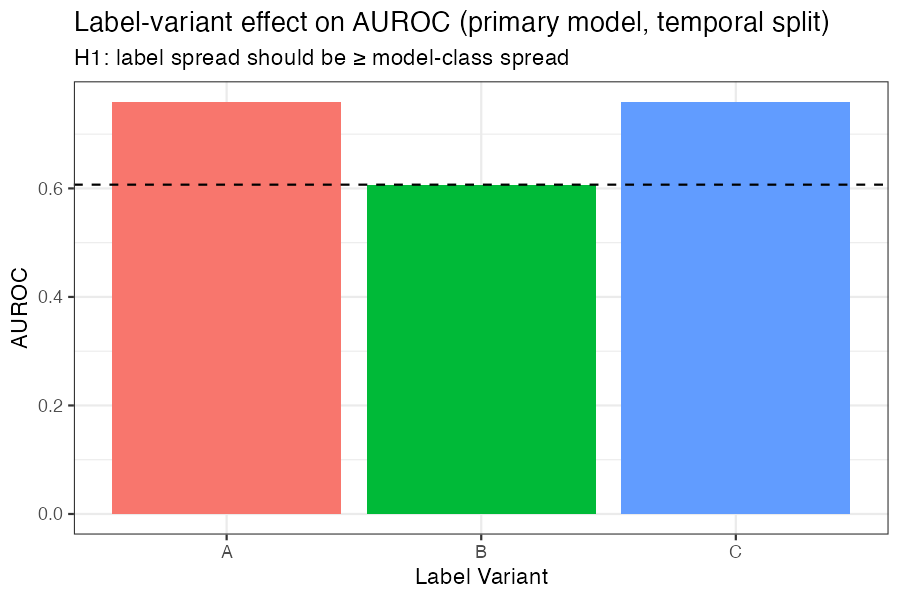
\includegraphics[width=\textwidth]{images/09_label_variance_auroc.png}
\end{column}
\begin{column}{0.48\textwidth}
  \begin{itemize}
    \item \textbf{Label variation:} AUROC changed by \textbf{0.153} when the sepsis definition changed while using the same model.
    \item \textbf{Model variation:} AUROC changed by \textbf{0.145} when the model changed while using the same label.
    \item This confirms Cohen et al.'s~\cite{cohen2024subtle} finding that sepsis label definition can strongly influence model performance.
  \end{itemize}
  \vspace{4pt}
  \begin{alertblock}{}
    The way sepsis is defined can affect performance as much as, or more than, the AI model itself.
  \end{alertblock}
\end{column}
\end{columns}
\end{frame}

%========================================================================================
% VI. RESULTS — H2: COEFFICIENT INSTABILITY
%========================================================================================
\begin{frame}{VI. Results --- H2: Coefficient Instability {\small\color{BabyMint!60!green}(CONFIRMED)}}
\begin{itemize}
  \item \textbf{10 out of 25 features} changed their effect or strength significantly across different sepsis label definitions.
  \item Affected features include: MAP, temperature, bilirubin, platelets, vasopressors, norepinephrine/epinephrine, respiratory rate change, platelet measurement, WBC measurement, and P/F ratio.
\end{itemize}

\vspace{6pt}
\begin{block}{Implication}
  A published hazard ratio for MAP could show a positive, negative, or almost no association with sepsis risk depending only on how the antibiotic-culture time window is defined~\cite{lauritsen2021framing}.
\end{block}

\vspace{6pt}
\textbf{Feature effects cannot be reliably interpreted without knowing which sepsis label definition was used.}
\end{frame}

%========================================================================================
% VI. RESULTS — H3: TREATMENT LEAKAGE
%========================================================================================
\begin{frame}{VI. Results --- H3: Treatment Leakage {\small\color{BabyMint!60!green}(CONFIRMED)}}
The treatment-anchored window~\cite{kamran2024evaluation} uses only information available \textbf{before the first antibiotic or blood culture}.

\vspace{6pt}
\begin{columns}[c]
\begin{column}{0.40\textwidth}
\begin{center}
\tablestyle
\begin{tabular}{lc}
\toprule
\textbf{Metric} & \textbf{Value} \\
\midrule
Patient-hours analysed & 179,003 \\
Sepsis onset events    & \textbf{0} \\
\bottomrule
\end{tabular}
\end{center}
\end{column}
\begin{column}{0.58\textwidth}
\begin{alertblock}{Critical Finding}
  No sepsis onset event is found before the clinical actions used to define the Sepsis-3 label.
\end{alertblock}
\end{column}
\end{columns}

\vspace{6pt}
This is not just a small drop in model performance (0.03 AUROC). The prediction target is \textbf{completely missing} in the clinically realistic time window.

\vspace{4pt}
\textbf{Most MIMIC-IV sepsis prediction models are learning when doctors suspect sepsis and start treatment, rather than detecting when a patient's health is starting to get worse.}
\end{frame}

%========================================================================================
% VI. RESULTS — H4: SPLIT OPTIMISM
%========================================================================================
\begin{frame}{VI. Results --- H4: Split Optimism {\small\color{BabyMint!60!green}(CONFIRMED)}}
\begin{center}
\tablestyle
\begin{tabular}{llcc}
\toprule
\textbf{Split} & \textbf{Model} & \textbf{AUROC} & \textbf{Utility Score} \\
\midrule
Temporal & Primary & 0.607 & --1.004 \\
Random   & Primary & 0.730 & --1.000 \\
Temporal & GBT     & 0.746 & --4.849 \\
Random   & GBT     & 0.720 & --5.167 \\
\bottomrule
\end{tabular}
\end{center}

\vspace{6pt}
\begin{itemize}
  \item \textbf{Primary model:} Random-split AUROC was \textbf{0.123 higher} than temporal-split AUROC (threshold: $\geq$ 0.02).
  \item The random split lets future patient patterns leak into training, inflating reported performance.
  \item This confirms Guo et al.'s~\cite{guo2022temporal} finding: \textbf{studies using random splits may overestimate real-world performance.}
\end{itemize}
\end{frame}

%========================================================================================
% VI. RESULTS — H5: EXTERNAL VALIDATION
%========================================================================================
\begin{frame}{VI. Results --- H5: External Validation on eICU-CRD~\cite{pollard2018eicu}}
\begin{center}
\tablestyle
\begin{tabular}{llccc}
\toprule
\textbf{Variant} & \textbf{Model} & \textbf{AUROC (eICU)} & \textbf{AUROC (MIMIC)} & \textbf{Drop} \\
\midrule
A & Primary & 0.736 & 0.760 & 0.024 \\
B & Primary & \textbf{0.437} & 0.607 & \textbf{0.170} \\
C & Primary & 0.725 & 0.759 & 0.034 \\
--- & NEWS2 & 0.605 & 0.63 & 0.025 \\
\bottomrule
\end{tabular}
\end{center}

\vspace{6pt}
\begin{itemize}
  \item Variants A and C showed similar performance on both datasets, with only small drops.
  \item \textbf{Variant B (Seymour-Standard) showed a large performance drop of 0.170 AUROC} when tested on eICU-CRD.
  \item The most commonly used sepsis label definition did not transfer well to a different hospital dataset.
\end{itemize}
\end{frame}

%========================================================================================
% VI. RESULTS — H6: MODEL-CLASS DIFFERENCE
%========================================================================================
\begin{frame}{VI. Results --- H6: Model-Class Difference {\small\color{BabyPink!70!red}(REJECTED)}}
\begin{columns}[c]
\begin{column}{0.50\textwidth}
  \centering
  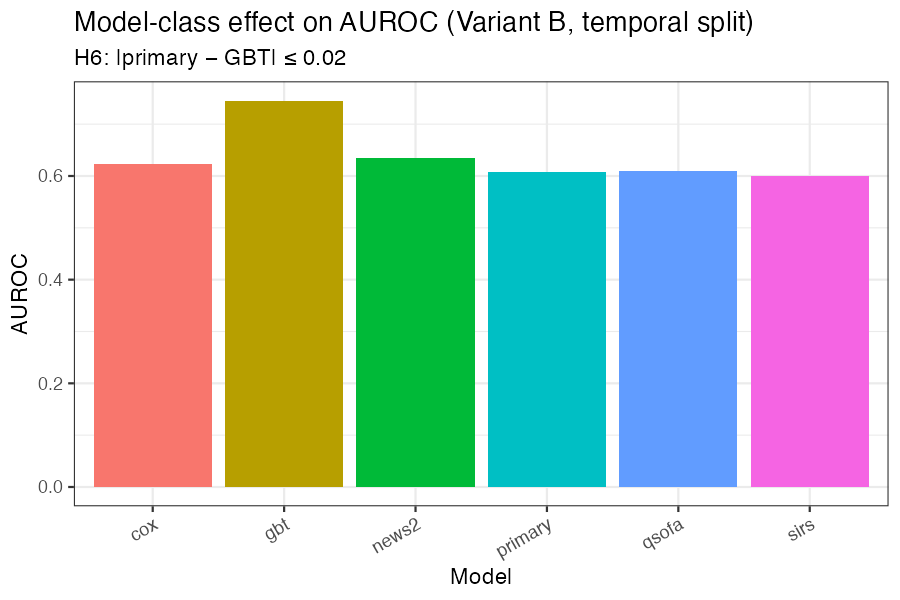
\includegraphics[width=\textwidth]{images/09_model_class_auroc.png}
\end{column}
\begin{column}{0.48\textwidth}
  \begin{itemize}
    \item \textbf{GBT AUROC:} 0.746
    \item \textbf{Primary Model AUROC:} 0.607
    \item Difference: \textbf{0.139}
  \end{itemize}
  \vspace{4pt}
  \begin{itemize}
    \item \textbf{GBT Utility Score:} --4.849
    \item \textbf{Primary Utility Score:} --1.004
  \end{itemize}
  \vspace{6pt}
  \begin{alertblock}{}
    The model ranking changes depending on the evaluation metric. A model that looks better by AUROC may perform worse in real clinical use.
  \end{alertblock}
\end{column}
\end{columns}
\end{frame}

%========================================================================================
% VI. RESULTS — INTERNAL PERFORMANCE
%========================================================================================
\begin{frame}{VI. Results --- Internal Performance (Temporal Test)}
\begin{center}
\tablestyle
\begin{tabular}{llccc}
\toprule
\textbf{Variant} & \textbf{Model} & \textbf{AUROC} & \textbf{Utility Score} & \textbf{Alert Burden} \\
\midrule
A & Primary & 0.760 & \textbf{--1.000} & $\infty$ \\
A & GBT     & 0.742 & --4.667 & 203 \\
B & Primary & 0.607 & --1.004 & $\infty$ \\
B & \textbf{GBT} & \textbf{0.746} & --4.849 & 194 \\
C & Primary & 0.759 & --1.000 & $\infty$ \\
C & GBT     & 0.752 & --2.475 & 93 \\
--- & NEWS2 & 0.63--0.64 & --1.1 to --1.6 & 97--223 \\
\bottomrule
\end{tabular}
\end{center}

\vspace{6pt}
\textbf{All models had a negative Utility Score}, meaning they did not provide clinical benefit and performed worse than giving no alerts.

\vspace{3pt}
\textbf{Alert burden:} For every real sepsis alert, the system generated \textbf{93--359 false alerts} (benchmark: 1.4~\cite{moor2023review}).
\end{frame}

%========================================================================================
% VI. RESULTS — EQUITY ANALYSIS
%========================================================================================
\begin{frame}{VI. Results --- Equity Analysis {\small\color{BabyLavender!70!blue}(Novel Finding)}}
\begin{columns}[c]
\begin{column}{0.48\textwidth}
  \centering
  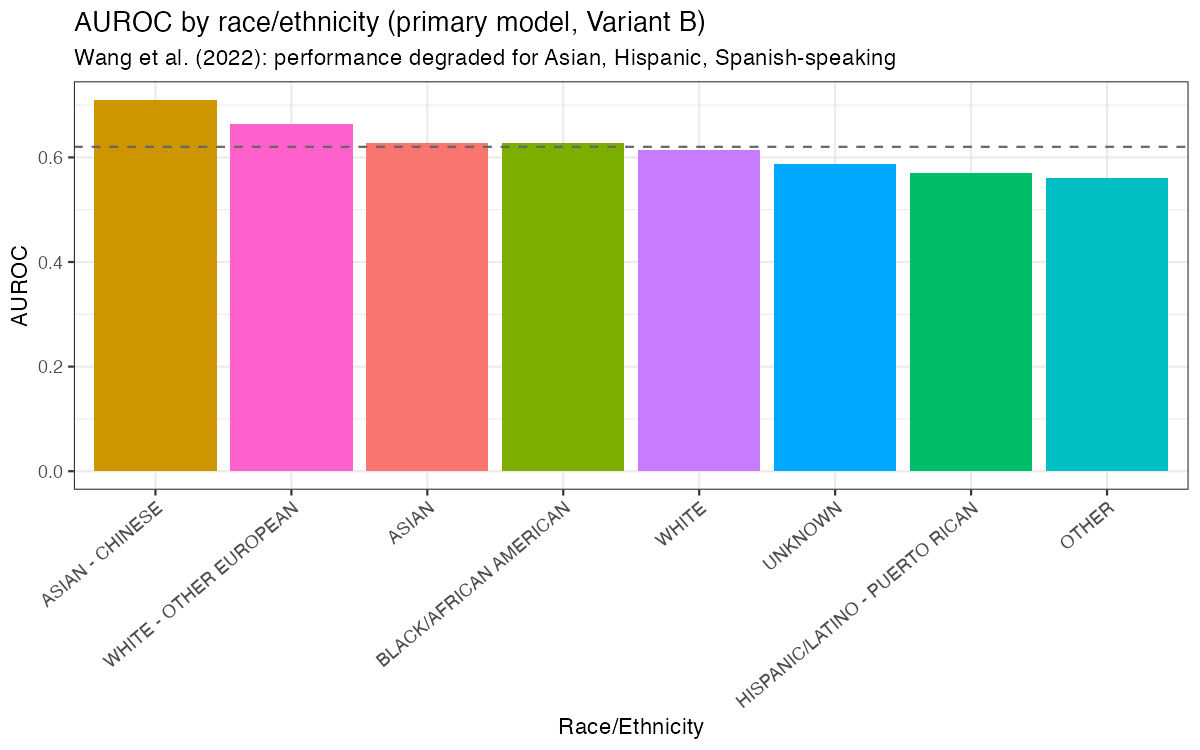
\includegraphics[width=\textwidth]{images/10_auroc_by_race.png}
\end{column}
\begin{column}{0.50\textwidth}
  \begin{itemize}
    \item AUROC varied by up to \textbf{0.15} across racial subgroups (primary model, Variant~B), from 0.56 (Other) to 0.71 (Asian-Chinese).
    \item The percentage of patients labelled as septic changed by \textbf{7.4--14.2 percentage points} across different label definitions within demographic subgroups.
    \item The \textbf{Unknown/Unable-to-obtain} race groups showed the largest changes (12.3--12.8\,pp).
    \item This is the first study to examine both model performance disparities and label sensitivity across subgroups~\cite{wang2022equity}.
  \end{itemize}
\end{column}
\end{columns}
\end{frame}

%========================================================================================
% VI. RESULTS — VARIANCE DECOMPOSITION SUMMARY
%========================================================================================
\begin{frame}{VI. Results --- Variance Decomposition Summary}
\begin{center}
\tablestyle
\begin{tabular}{lccc}
\toprule
\textbf{Factor} & \textbf{AUROC Change} & \textbf{Related Hypothesis} & \textbf{Status} \\
\midrule
Sepsis label definition & 0.153 & H1 & \textcolor{BabyMint!60!green}{\textbf{CONFIRMED}} \\
Model choice & 0.145 & H6 & \textcolor{BabyPink!70!red}{\textbf{REJECTED}} \\
Split method (temporal vs random) & 0.123 & H4 & \textcolor{BabyMint!60!green}{\textbf{CONFIRMED}} \\
Evaluation metric (AUROC vs Utility Score) & 0.170 & H5 & --- \\
\bottomrule
\end{tabular}
\end{center}

\vspace{8pt}
\textbf{All four analyst decisions create AUROC changes of 0.12--0.17.}

\vspace{4pt}
Most studies fix one sepsis label and compare models. This measures only one source of variation while ignoring three other sources of similar importance.
\end{frame}

%========================================================================================
% VII. DISCUSSION — KEY FINDING
%========================================================================================
\begin{frame}{VII. Discussion --- Key Finding}
The performance collapse reported by Wang et al.~\cite{wang2025srpm} is not only a model evaluation issue. This study shows that it is strongly related to how the sepsis label is constructed.

\vspace{6pt}
\textbf{The Sepsis-3 label in MIMIC-IV has three important limitations:}
\begin{enumerate}
  \item \textbf{Depends on clinical actions} --- No sepsis cases are identified before treatment starts~\cite{kamran2024evaluation}.
  \item \textbf{Sensitive to label definition} --- Different reasonable interpretations can produce almost double the number of sepsis cases~\cite{cohen2024subtle}.
  \item \textbf{Produces poor clinical utility} --- All tested models show negative Utility Scores~\cite{wang2025srpm}.
\end{enumerate}

\vspace{6pt}
\begin{alertblock}{}
  \centering These findings suggest that improving model complexity alone cannot solve the problem. Better sepsis label design is required.
\end{alertblock}
\end{frame}

%========================================================================================
% VII. DISCUSSION — CONTRIBUTIONS
%========================================================================================
\begin{frame}{VII. Discussion --- Contributions}
\tablestyle
\begin{center}
\begin{tabular}{cp{12cm}}
\toprule
\textbf{\#} & \textbf{Contribution} \\
\midrule
C1 & Compared three different Sepsis-3 label definitions using the same prediction model on MIMIC-IV~\cite{cohen2024subtle}. \\
C2 & Showed that no sepsis cases exist before antibiotics or culture tests, highlighting that the label depends on clinical actions~\cite{kamran2024evaluation}. \\
C3 & Confirmed that all models had negative Utility Scores, extending the findings of Wang et al.~\cite{wang2025srpm}. \\
C4 & Found that 10 clinical features changed their effects across different label definitions, supporting Lauritsen et al.~\cite{lauritsen2021framing}. \\
C5 & Quantified split optimism: random splits inflated AUROC by 0.123 compared to temporal splits, confirming Guo et al.~\cite{guo2022temporal}. \\
C6 & First study to examine how different sepsis label definitions affect racial subgroup analysis~\cite{wang2022equity}. \\
C7 & Used a pre-registered, TRIPOD+AI-compliant, fully reproducible research pipeline~\cite{collins2024tripodai}. \\
\bottomrule
\end{tabular}
\end{center}
\end{frame}

%========================================================================================
% VII. DISCUSSION — LIMITATIONS
%========================================================================================
\begin{frame}{VII. Discussion --- Limitations}
\begin{itemize}
  \item \textbf{Small external event count:} The eICU dataset had only \textbf{63 sepsis cases}, making some evaluation metrics less reliable.
  \item \textbf{Deep learning comparison:} A deep survival model was planned but not implemented.
  \item \textbf{Limited features:} Clinical notes, procedure codes, and ventilator settings were not included.
  \item \textbf{Specific to Sepsis-3:} These findings apply to the Sepsis-3 label and may not apply to other sepsis definitions.
\end{itemize}

\vspace{8pt}
\begin{exampleblock}{}
  \centering These limits are documented rather than hidden.
\end{exampleblock}
\end{frame}

%========================================================================================
% VIII. CONCLUSION AND FUTURE WORK
%========================================================================================
\begin{frame}{VIII. Conclusion and Future Work}
\begin{enumerate}
  \item \textbf{Better sepsis labels:} Define sepsis using objective patient measurements (such as lactate levels and organ function) instead of treatment decisions.
  \item \textbf{Prospective study:} Test the new label in real clinical settings using future patient data.
  \item \textbf{Better alert threshold:} Choose the alert threshold that maximises clinical benefit (Utility Score) instead of only improving prediction accuracy.
  \item \textbf{Multi-hospital evaluation:} Test the model in different hospitals and identify an acceptable number of false alerts for clinical use.
\end{enumerate}
\end{frame}

%========================================================================================
% APPENDIX — LABEL SENSITIVITY
%========================================================================================
\begin{frame}{Appendix --- Label Sensitivity vs.\ AUROC}
\begin{center}
  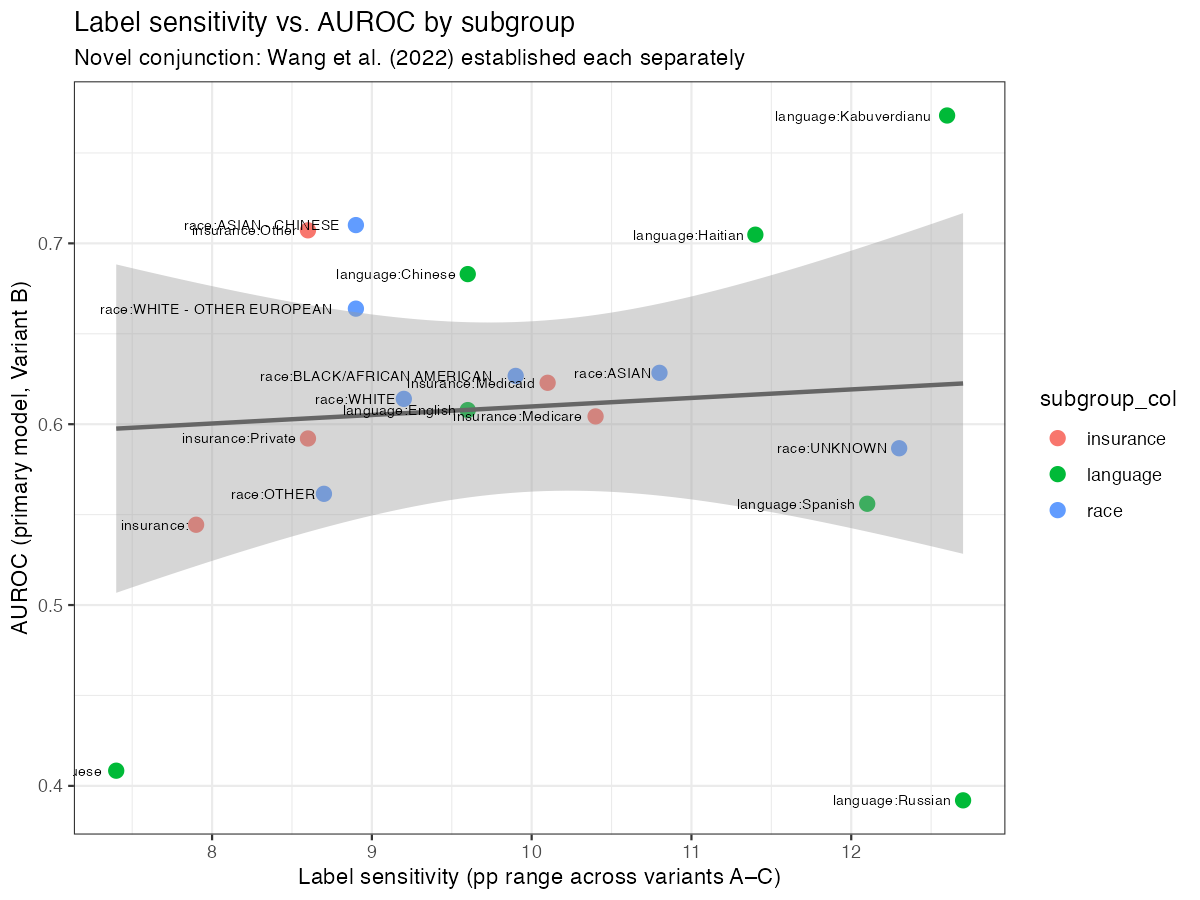
\includegraphics[height=0.80\textheight]{images/10_label_sens_vs_auroc.png}
\end{center}
\end{frame}

%========================================================================================
% REFERENCES
%========================================================================================
\begin{frame}[allowframebreaks]{References}
\scriptsize
\printbibliography[heading=none]
\end{frame}

%--- Thank You Slide ---
{
\setbeamertemplate{headline}{}
\setbeamertemplate{footline}{}
\begin{frame}[plain]
\begin{tikzpicture}[remember picture,overlay]
  \node[anchor=north west,inner sep=0pt] at (current page.north west) {%
    
\includegraphics[height=\paperheight]{images/leftbar.png}%
  };
  \fill[BabyBlue!10] ([xshift=1.8cm]current page.north west) rectangle ([yshift=-3cm]current page.north east);
  \draw[BabyPink,line width=1.5pt] ([xshift=1.8cm,yshift=-3cm]current page.north west) -- ([yshift=-3cm]current page.north east);
  \fill[BabyMint!10] ([xshift=1.8cm,yshift=2cm]current page.south west) rectangle (current page.south east);
  \draw[BabyLavender,line width=1pt] ([xshift=1.8cm,yshift=2cm]current page.south west) -- ([yshift=2cm]current page.south east);
  \node[anchor=north east] at ([xshift=-0.6cm,yshift=-0.3cm]current page.north east) {%
    
\includegraphics[width=2.8cm]{images/atu-logo-navy.png}%
  };
\end{tikzpicture}
\hspace{1.6cm}%
\begin{minipage}[t]{0.82\textwidth}
\vspace{1.5cm}
\begin{center}
  {\Huge\bfseries\color{DeepTeal} Thank You}\\[14pt]
  {\large\color{MidGrey} Questions \& Discussion}\\[18pt]
  {\normalsize\color{DarkText} Abdul Ahad}\\[4pt]
  {\small\color{MidGrey} ahadarif.1998@gmail.com}\\[4pt]
  {\small\color{MidGrey} Atlantic Technological University (ATU), Galway}
\end{center}
\end{minipage}
\end{frame}
}

\end{document}
